\documentclass[psamsfonts]{amsart}
\usepackage[utf8]{inputenc}
\usepackage[english]{babel}
 

\usepackage{amsmath}
\usepackage{enumitem}
\usepackage{mathrsfs}
\usepackage{amssymb}
\usepackage{amsthm}
\usepackage{multicol}
\usepackage{xr}
\usepackage{cancel}
\usepackage{graphicx}%
\usepackage{xfrac}
\usepackage{float}
%\usepackage[outer=2cm, inner=2cm]{geometry}
\usepackage{tikz}


\newtheorem*{remark}{Remark}
\newcommand{\pdx}{\frac{\partial f}{\partial x}}
\newcommand{\pdy}{\frac{\partial f}{\partial y}}
\newcommand{\pdz}{\frac{\partial f}{\partial z}}
\newcommand{\pdzz}{\frac{\partial f}{\partial \bar{z}}}
\newcommand{\C}{{\mathbb C}}       % Field of complex numbers
\newcommand{\Q}{{\mathbb Q}}       %
\newcommand{\R}{{\mathbb R}}       % Field of real numbers
\newcommand{\Prb}{{\mathbb P}} 
\newcommand{\E}{{\mathbb E}} 
\newcommand{\Rb}{{\overline{\mathbb R}}}
\newcommand{\ra}{\rightarrow} 
\newcommand{\N}{{\mathbb N}} 
\newcommand{\Z}{{\mathbb Z}} 
\newcommand{\stm}{{\setminus}} 
\newcommand{\vphi}{{\varphi}}
\newcommand{\A}{{\mathcal A}}
\newcommand{\U}{{\mathcal U}}
\newcommand{\M}{{\mathcal M}}
\newcommand{\D}{{\mathcal D}}
\newcommand{\Rec}{{\mathcal R}}
\newcommand{\h}{{\mathcal H}}
\newcommand{\cL}{{\mathcal L}}
\newcommand{\e}{{\varepsilon}}
\newcommand{\RA}{{\Rightarrow}}
\DeclareMathOperator{\diam}{diam}
\DeclareMathOperator{\dist}{dist}

%\DeclareMathOperator{\dim}{dim}
\def\ve{\varepsilon}
\newcommand{\sph}{{~~~~~~~~~~~~~}}
\newcommand{\cM}{{\mathcal M}}
\newcommand{\B}{{\mathcal B}}
\newcommand{\Po}{{\mathcal P}}
\theoremstyle{definition}
\newtheorem{thm}{Theorem}[section]
\newtheorem{defn}[thm]{Definition}
\newtheorem{lem}[thm]{Lemma}
\newtheorem{cor}[thm]{Corollary}
\newtheorem{prop}[thm]{Proposition}
\newtheorem{rem}[thm]{Remark}
\newtheorem{ex}[thm]{Example}
\newtheorem{recall}[thm]{Recall}
\newtheorem{nota}[thm]{Notation}
\usetikzlibrary{arrows,positioning} 
\tikzset{
    %Define standard arrow tip
    >=stealth',
    %Define style for boxes
    punkt/.style={
           circle,
           draw=black, thick,
           text width=2em,
           minimum height=2em,
           text centered},
    % Define arrow style
    pil/.style={
           ->,
           thick,
           shorten <=2pt,
           shorten >=2pt,}
}


%\DeclareMathOperator{\dim}{dim}
\def\ve{\varepsilon}

\title{Efficient Coupling for Finite State Markov Chains: 
Chains Without Efficient Coupling}
\author{Iddo Ben-Ari and Rachel Lonchar}

\begin{document}
\maketitle
 





%Iddos notes
%
%
%\section{Abstract} 
\begin{ex}
Using the ``switch'' idea from Corollary 3.3, we can develop a Markov chain with only three states that will not have an efficient (Markovian component exchangeable) coupling. Figure \ref{F1}, shows ones such chain. 
\begin{figure}
\centering
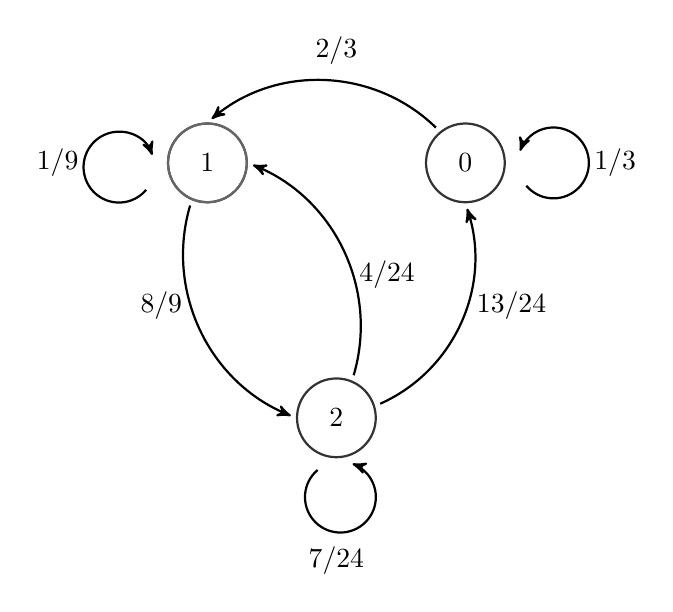
\begin{tikzpicture}[
rno/.style={circle, draw=black!80, fill=green!0,  thick, minimum size=10mm},
rnoin/.style={circle, draw=black!60,   thick, minimum size=10mm},
 % Define arrow style
    pil/.style={
           ->,
           thick,
           shorten <=2pt,
           shorten >=2pt,}
]
%Nodes
\draw[thick, <-] (-.7,.1) arc (20:320:.45);
\draw[thick, ->] (4.05,-.29) arc (220:520:.45);
\draw[thick, ->] (1.4,-3.9) arc (130:430:.45);
\node[rno] (main1) {1};
\node (branch11) [left= of main1] {1/9};
\node (dum1) [right=of main1] {};
\node[rno] (main0) [right= of dum1] {0}
edge[pil, bend right=42] (main1.north);
\node (dum2) [below= of main1] {8/9~~~~~~~~~~~};
\node (dum6) [below= of dum1] {~~~~~~~~~~~4/24};
\node (dum3) [below= of main0] {~~~~~~~~~~13/24};
\node (branch01) [above=of dum1] {2/3};
\node (dum4) [below= of dum2] {};
\node[rno] (main2) [below= of dum6] {2}
edge[pil, bend right=42] (main1.east)
edge[pil, bend right=42] (main0.south);
\node (dum5) [below= of dum3] {};
\node[rnoin] (ghost1) [=of main1] {}
edge[pil, bend right=42] (main2.west);
\node (branch00) [right= of main0] {1/3};
\node (branch22) [below= of main2] {7/24};
\end{tikzpicture}
\caption{A three-state chain without efficient coupling.} \label{F1}
\end{figure}

\end{ex} 
\begin{ex}
Using the ``switch'' idea from Corollary 3.3, we can develop a Markov chain with only three states that will not have an efficient (Markovian component exchangeable) coupling. Figure \ref{F1}, shows ones such chain. 
\begin{figure}
\centering
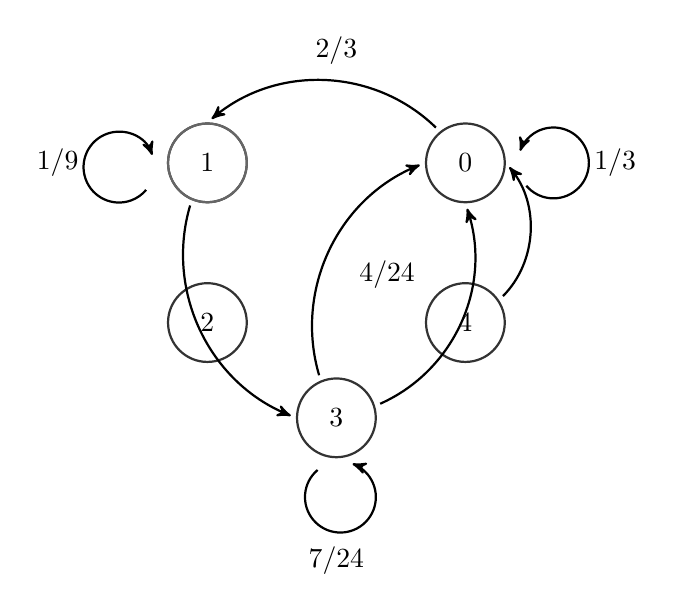
\begin{tikzpicture}[
rno/.style={circle, draw=black!80, fill=green!0,  thick, minimum size=10mm},
rnoin/.style={circle, draw=black!60,   thick, minimum size=10mm},
 % Define arrow style
    pil/.style={
           ->,
           thick,
           shorten <=2pt,
           shorten >=2pt,}
]
%Nodes
\draw[thick, <-] (-.7,.1) arc (20:320:.45);
\draw[thick, ->] (4.05,-.29) arc (220:520:.45);
\draw[thick, ->] (1.4,-3.9) arc (130:430:.45);
\node[rno] (main1) {1};
\node (branch11) [left= of main1] {1/9};
\node (dum1) [right=of main1] {};
\node[rno] (main0) [right= of dum1] {0}
edge[pil, bend right=42] (main1.north);
\node[rno] (dum2) [below= of main1] {2};
\node (dum6) [below= of dum1] {~~~~~~~~~~~4/24};
\node[rno] (dum3) [below= of main0] {4}
edge[pil, bend right=42] (main0.east);
\node (branch01) [above=of dum1] {2/3};
\node (dum4) [below= of dum2] {};
\node[rno] (main2) [below= of dum6] {3}
edge[pil, bend left=42] (main0.west)
edge[pil, bend right=42] (main0.south);
\node (dum5) [below= of dum3] {};
\node[rnoin] (ghost1) [=of main1] {}
edge[pil, bend right=42] (main2.west);
\node (branch00) [right= of main0] {1/3};
\node (branch22) [below= of main2] {7/24};
\end{tikzpicture}
\caption{A three-state chain without efficient coupling.} \label{F1}
\end{figure}

\end{ex} 

\begin{figure}
\centering
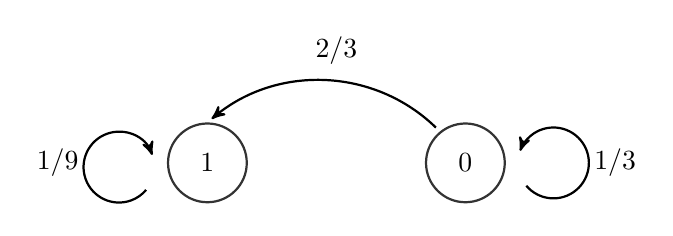
\begin{tikzpicture}[
rno/.style={circle, draw=black!80, fill=green!0,  thick, minimum size=10mm},
rnoin/.style={circle, draw=black!60,   thick, minimum size=10mm},
 % Define arrow style
    pil/.style={
           ->,
           thick,
           shorten <=2pt,
           shorten >=2pt,}
]
%Nodes
\draw[thick, <-] (-.7,.1) arc (20:320:.45);
\draw[thick, ->] (4.05,-.29) arc (220:520:.45);
%\draw[thick, ->] (1.4,-3.9) arc (130:430:.45);
\node[rno] (main1) {1};
\node (branch11) [left= of main1] {1/9};
\node (dum1) [right=of main1] {};
\node[rno] (main0) [right= of dum1] {0}
edge[pil, bend right=42] (main1.north);
\node (branch01) [above=of dum1] {2/3};
\node (branch00) [right= of main0] {1/3};
%\node (branch22) [below= of main2] {7/24};
\end{tikzpicture}
\caption{A three-state chain without efficient coupling.} \label{F1}
\end{figure}







\end{document}
